\documentclass{article}
\usepackage[utf8x]{inputenc}
\usepackage[colorlinks=true,linkcolor=black,citecolor=blue,pdfusetitle,pagebackref=false]{hyperref}
\usepackage[nonumberlist]{glossaries}
\usepackage{graphicx}
\usepackage{multicol}
\usepackage{caption}
\usepackage{subcaption}
\usepackage{amsmath}
\usepackage{bm}
\usepackage[margin=1.5cm]{geometry}
\usepackage{cite}
\usepackage[usenames,dvipsnames,svgnames,table]{xcolor}
\usepackage{bigints}

\newenvironment{Figure}
  {\par\medskip\noindent\minipage{\linewidth}}
  {\endminipage\par\medskip}

\bibliographystyle{unsrt}
\renewcommand\refname{References}

\newacronym{cdi}
    {CDI}{coherent diffractive imaging}

\newacronym{odt}
    {ODT}{optical dipole trap}

\newacronym{bec}
    {BEC}{Bose-Einstein condensate}

\newacronym{fort}
    {FORT}{far-off-resonance trap}

\newacronym{ta}
    {TA}{tapered amplifier}

\newacronym{caes}
    {CAES}{cold-atom electron source}

\newacronym{xfel}
    {XFEL}{x-ray free electron laser}

\newacronym{mot}
    {MOT}{magneto-optical trap}

\newacronym{ecdl}
    {ECDL}{external cavity diode laser}

\newacronym{aom}
    {AOM}{acousto-optical modulator}

\newacronym{slm}
    {SLM}{spatial light modulator}

\newacronym{mopa}
    {MOPA}{master-oscillator power amplifier}

\newacronym{na}
    {NA}{numerical aperture}

\newacronym{ar}
    {AR}{anti-reflection}

\newacronym{ccd}
    {CCD}{charge-coupled device}

\newacronym{cro}
    {CRO}{cathode ray oscilloscope}

\newacronym{pbs}
    {PBS}{polarising beam splitter}

\newacronym{bs}
    {BS}{beam splitter}

\newacronym{npbs}
    {NPBS}{non-polarising beam splitter}

\newacronym{tec}
    {TEC}{thermo-electric cooler}

\newacronym{cw}
    {CW}{continuous wave}

\newacronym{mcp}
    {MCP}{microchannel plate}

\newacronym{fwhm}
    {FWHM}{full-width half maximum}

\newacronym{pdh}
    {PDH}{Pound-Drever-Hall}
    
\newacronym{ps}
    {PS}{polarisation spectroscopy}
    
\newacronym{obe}
    {OBE}{optical Bloch equation}
    
\newacronym{davll}
    {DAVLL}{dichroic atomic vapour laser lock}

\newacronym{mts}
    {MTS}{modulation transfer spectroscopy}

\newacronym{snr}
    {SNR}{signal-to-noise ratio}

\newacronym{lsd}
    {LSP}{linear spectral density}


\makeglossaries

\begin{document}
\title{Maybe sub-kHz Linewidths using Polarisation Spectroscopy}
\author{Joshua Torrance}

\maketitle

\begin{abstract}
By capitalising on the demonstrably high bandwidth of polarisation spectroscopy locking systems it it possible to achieve linewidths of 15 kHz using standard diode lasers.
\end{abstract}

\begin{multicols}{2}

\section{Introduction}
Laser frequency stabilisation is essential to numerous applications such as the cooling and trapping of atoms, optical fibre communications and metrology\cite{metcalf_laser_1999, demtroder_laser_2014}. Polarisation spectroscopy has much in common with the standard laser locking techinique, saturated absorption spectroscopy\cite{maguire_theoretical_2006, haroche_theory_1972, preston_doppler-free_1996} as both techniques provide a frequency reference that can be used to lock lasers to atomic resonaces.

{\color{red}Narrow linewidth is good...}

Narrow linewidth lasers are important for applications in metrology\cite{ye_quantum_2008}, atomic clocks\cite{ludlow_sr_2008}, atomic trapping and cooling\cite{uetake_high_2008, ye_stable_2010, akamatsu_narrow_2012} and high resolution spectroscopy\cite{rafac_sub-dekahertz_2000}.

{\color{red}Current linewidths are...}

Current techniques for minimising laser linewidths range from simple laser stabilisation with saturated absorption, which can achieve linewidths in the region of 150kHz\cite{cuneo_optically_1994}, to elaborate experiments involved extremely high finesse cavities that are able to achieve sub-Hertz linewidths with diode lasers using \gls{pdh} locking.\cite{ludlow_compact_2007}

{\color{red}History...}

Polarisation spectroscopy was first presented as an alternative to saturated absorption spectroscopy with higher signal to noise ratios\cite{wieman_doppler-free_1976}. Later developments on the technique use a balanced polarimeter instead of crossed polarisers in order to obtain a background-free dispersion signal which is suitable for high-speed and more robust stabilisation\cite{yoshikawa_frequency_2003}.

{\color{red}Phase stabilisation dipole response time}

Polarisation spectroscopy can be used for phase stabilisation due to the finite response time of the atomic dipoles to pertubation in the laser phase\cite{torii_laser-phase_2012}. {\color{red} I don't like this sentence. Also what about response time of sub-level population? Similar to \cite{pearman_polarization_2002} although that one is static not dynamic. What's the response time for sub-level population response?}

{\color{red}Description of pol spec with reference to papers that explain it in detail.}

{\color{red}Experimental setup}

A schematic diagram of the experimental setup can be seen in figure \ref{polspec_schematic}. An \gls{ecdl} (Toptica DL Pro) operating at 780nm with {\color{red} a diode of some description} which outputs {\color{red}X} mW. This light is then split by a \gls{pbs} and the light transmitted through the \gls{pbs} passes through a \gls{aom} twice before entering a fibre to the cavity linewidth setup as shown in figure \ref{cavity_schematic}. The light reflected through the \gls{pbs} goes through an optical fibre to the polarisation specroscopy setup shown in figure \ref{polspec_schematic}.

\begin{Figure}
    \centering
    \captionsetup{type=figure}
    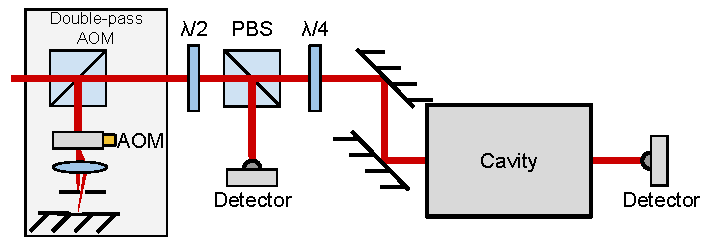
\includegraphics[width=\linewidth]{Figs/CavityLinewidth.pdf}
    \captionof{figure}{A simplified schemeatic diagram of the cavity setup used to measure linewidth.}
    \label{cavity_schematic}
\end{Figure}

\begin{Figure}
    \centering
    \captionsetup{type=figure}
    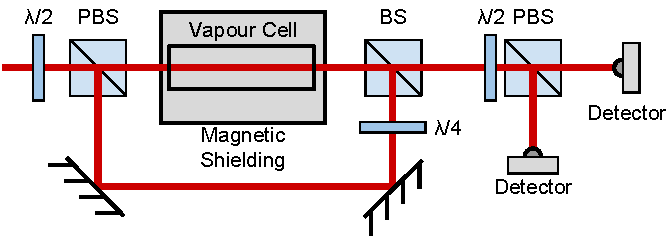
\includegraphics[width=\linewidth]{Figs/PolSpec.pdf}
    \captionof{figure}{A simplified schematic diagram of the polarisation spectroscopy setup.}
    \label{polspec_schematic}
\end{Figure}

{\color{red}Bandwidth (and data)}

{\color{red}Phase lead? (and details and data)}

{\color{red}Linewidth measurement (and data)}

{\color{red}Conclusion}

\section{Papers}
\begin{itemize}
    \item Oringal Wieman and H\"ansch paper\cite{wieman_doppler-free_1976}.
    \item Analogy to PDH explaining phase memory and fast response in \cite{torii_laser-phase_2012}.
    \item Mathematics on polarisation rotation through the sample and simulation of pumping transitions in \cite{pearman_polarization_2002}.
    \item Bloch equations to population anisotropy\cite{harris_polarization_2006}
    \item `Bi-polarisation spectroscopy' two pairs of beams through sample\cite{tiwari_laser_2006}.
    \item Rate equations used to calculate spectra and good comparison to experiment\cite{do_polarization_2008}.
\end{itemize}


\section{Polarisation Spectroscopy Theory}

Simplistic view:
\begin{itemize}
    \item Circular pump beam travels through the sample.
    \item When the frequency is tuned to a transition the atoms are pumped to a magnetic substate.
    \item The linearly polarised probe beam can be decomposed into $\sigma$\textsuperscript{+} and $\sigma$\textsuperscript{-}. Each of these components experience a differenct absorption coefficient and different refractive indices from the nonisotropic saturation of the magnetic sublevels caused by the pump. This results in the probe beam becoming eliptically polarised and rotating the major axis.
    \item This rotation is easily observed by the analyser.
\end{itemize}

\begin{Figure}
    \centering
    \captionsetup{type=figure}
    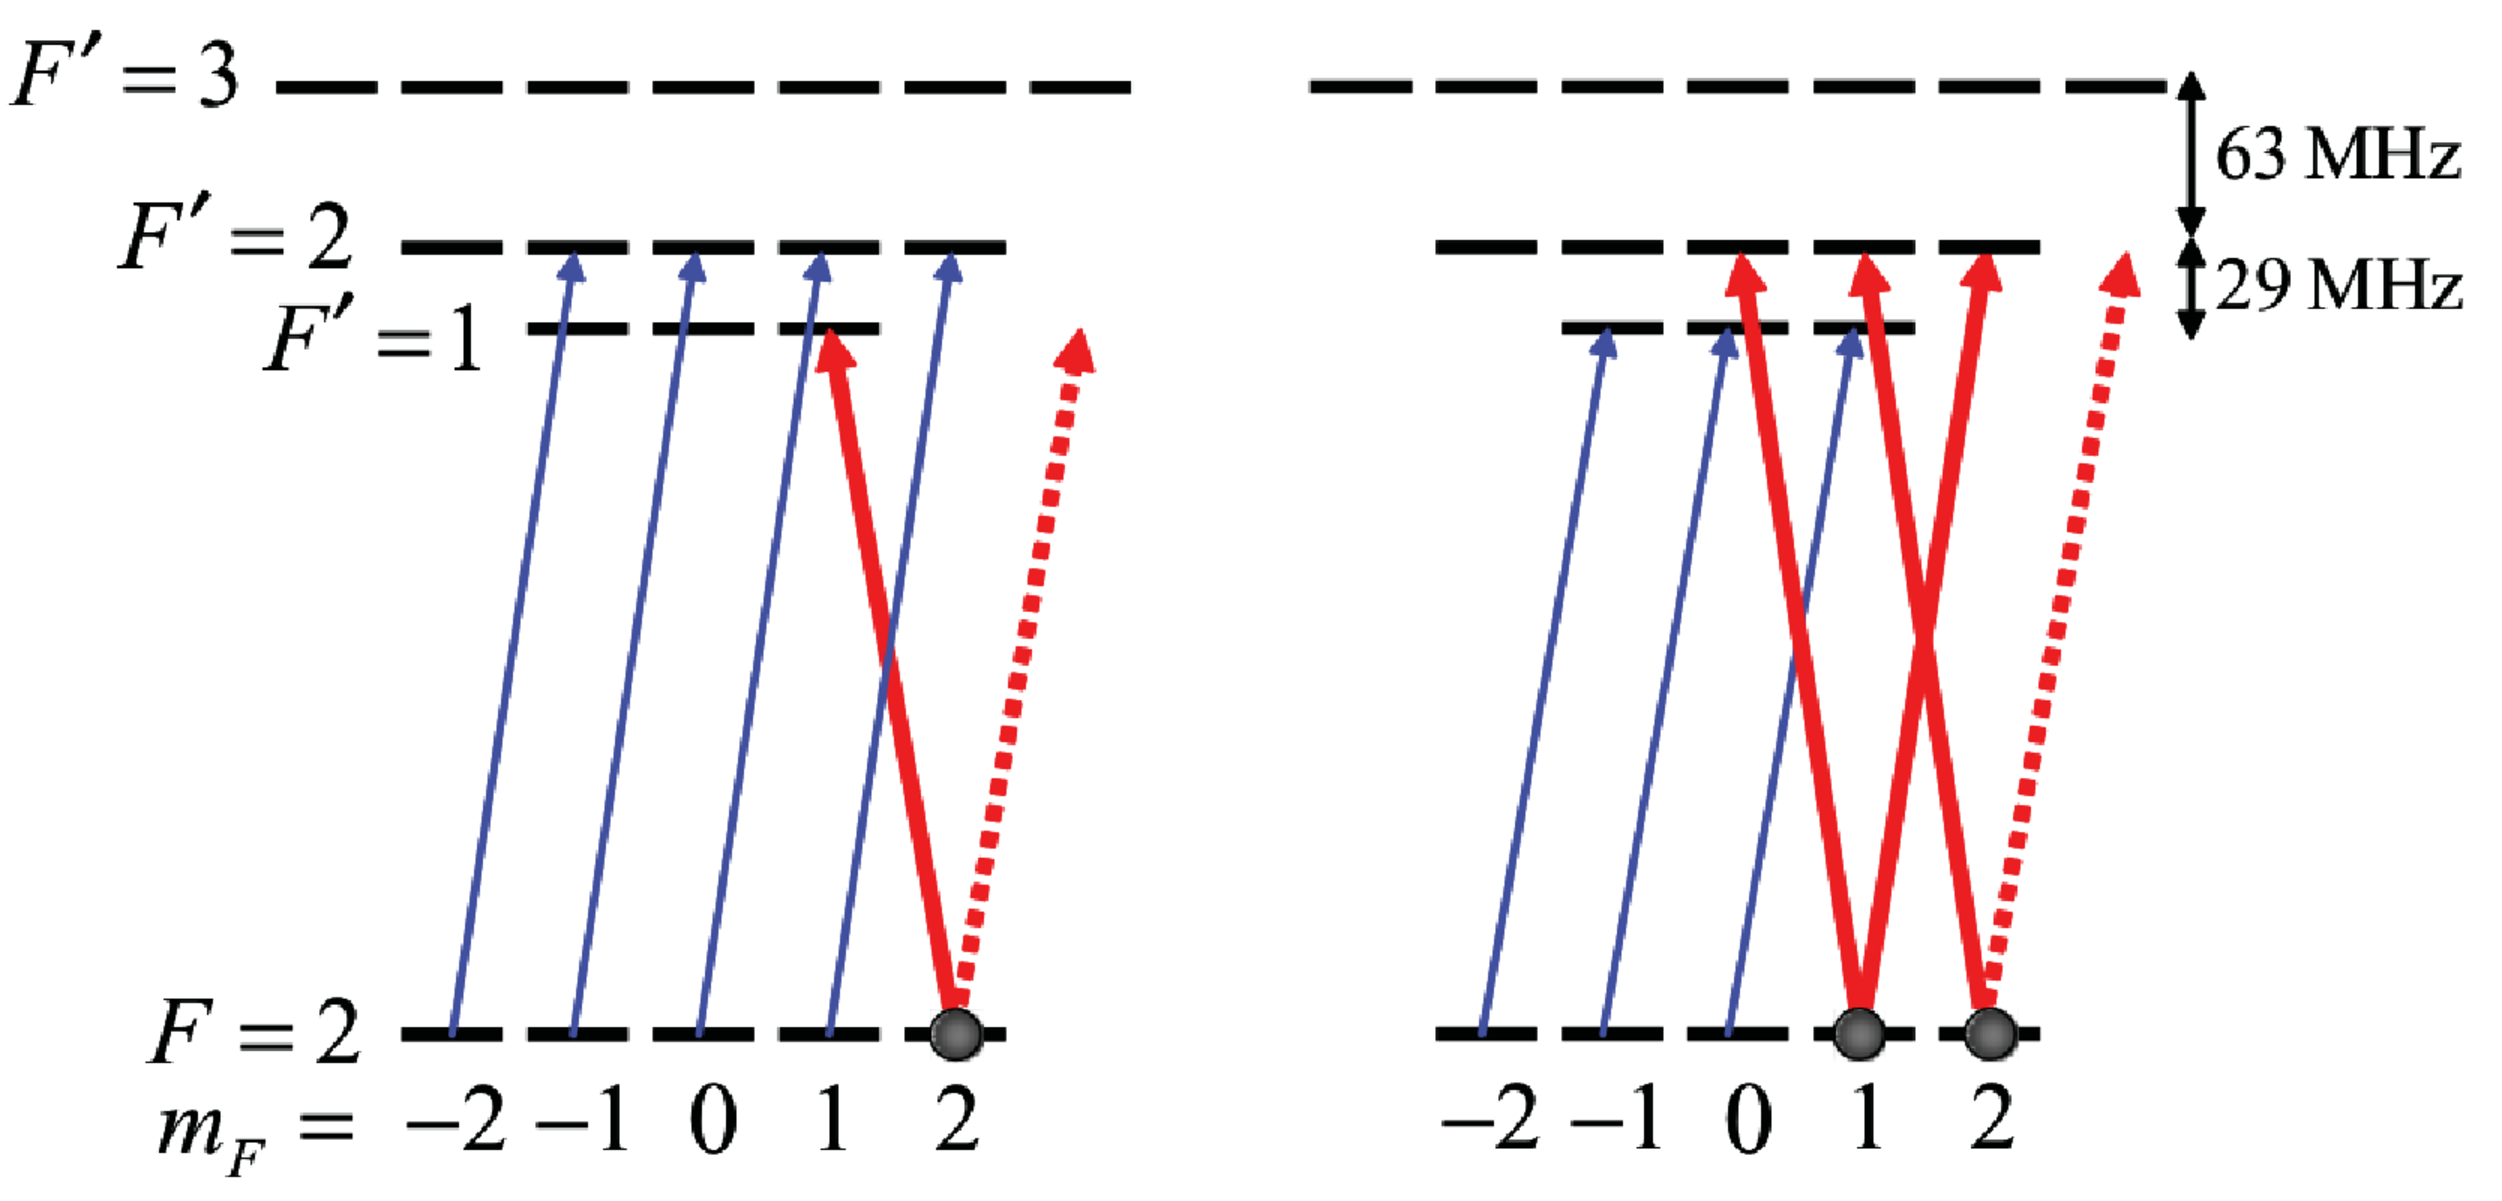
\includegraphics[width=\linewidth]{Figs/splitenergylevels.pdf}
    \captionof{figure}{Two pump probe configurations contributing to the crossover transition. The blue thin arrows indicate the transitions by the $\sigma^+$ pump (spin-polarising) beam which optically pumps the atom to the $m_F=1$ or $m_F=2$ states. The red thick arrows indicate the transitions by the probe beam. The $\sigma^+$ transitions which are not allowed for the pin-polarised atom are indicated by the red dotted arrows. In both configurations, the $\sigma^-$ component of the probe beam predominantly interacts with the atoms, resulting in circular birefringence for the probe beam.}
    \label{simulationfigure}
\end{Figure}

\subsection{Birefringence in the Atomic Sample}
The initial state of the probe beam with linear polarisation in a plane at an angle $\phi$ from the $x$ axis can be expressed as
\begin{equation}
\bm{E} = \begin{bmatrix} E_x \\ E_y \end{bmatrix} = E_0 \begin{bmatrix} \cos \phi \\ \sin \phi \end{bmatrix}.
\end{equation}

This can be reexpressed in terms of the circular polarisation basis vectors
\begin{equation}
\bm{E} = E_0 \begin{bmatrix} \cos \phi \\ \sin \phi \end{bmatrix} = E_0 \left \{ \frac{e^{-i\phi}}{2} \begin{bmatrix} 1 \\ i \end{bmatrix} + \frac{e^{i\phi}}{2} \begin{bmatrix} 1 \\ -i \end{bmatrix} \right \}
\end{equation}

After the beam has passed through the cell windows and atomic sample the electric field of the probe is
\begin{align}
\begin{split}
\bm{E} = E_0 \Biggl\{ &\frac{e^{-i\phi}}{2}\begin{bmatrix} 1 \\ i \end{bmatrix}e^{-ik_+L} e^{-\alpha_+L/2} e^{-ik_{w+}l} \;+ \\
&\frac{e^{i\phi}}{2}\begin{bmatrix} 1 \\ -i \end{bmatrix}e^{-ik_-L} e^{-\alpha_-L/2} e^{-ik_{w-}l} \Biggr\}
\end{split}
\end{align}
where $k_\pm = \frac{\omega}{c}n_\pm$, $n_\pm$ are the refractive indices of the gas for the circular polarisation components which drive $\sigma_\pm$ transitions; $\alpha_\pm$ are the corresponding absorption cooefficients and the $k_\pm = \frac{w}{c}n_{w\pm}$ terms describe te phase change picked up while traversing the window (windows??) of width l. The refractive indices are complex and can be written as $n_{w\pm}l=b_{R\pm} - i\frac{c}{\omega}b_{l\pm}$. We can rewrite the expression as
\begin{align}\begin{split}
\bm{E} = E_0 \exp&\Biggl\{-i\Biggl[\frac{\omega}{c}(nL+b_R)-ib_l-i\frac{\alpha L}{2}\Biggr]\Biggr\} \\
&\Biggl\{\frac{e^{-i\phi}}{2}\begin{bmatrix} 1 \\ i\end{bmatrix} e^{+i\Omega} + \frac{e^{i\phi}}{2} \begin{bmatrix} 1 \\ -i \end{bmatrix} e^{-i\Omega} \Biggr\}.
\end{split}\end{align}

where,

\begin{align}\begin{split}
\Omega &= \frac{\omega}{2c}(\Delta n L + \Delta b_R) - i\left(\frac{L}{4}\delta\alpha _ \frac{1}{2}\delta b_l \right), \\
n &= \frac{1}{2}(n_+ + n_-),\\
\alpha &= \frac{1}{2}(\alpha_+ + \alpha_-), \\
b_R &= \frac{1}{2}(b_{R+} + b_{R-}),\\
b_l &= \frac{1}{2}(b_{l+} + b_{l-}) \\
\Delta n &= n_+ - n_-,\\
\Delta \alpha &= \alpha_+ - \alpha_-,\\
\Delta b_R &= b_{R+} - n_{R-},\\
\Delta b_l &= b_{l+} - b_{l-}.
\end{split}\end{align}

The polarising beam splitter cube in the analyser will split the probe beam into its horizontal ($x$) and vertical ($y$) components and the difference in intensity gives the polarisation spectroscopy signal:

\begin{align}\begin{split}
I_{signal} &= I_y - I_x\\
I_{signal} &= I_0 e^{-\alpha L - 2b_l} \cos\left(2\phi + L \Delta n \frac{\omega}{c} + \Delta b_R\frac{\omega}{c} \right)
\end{split}\end{align}

Here, $I_0$ is the intensity of the probe beam before the cell.

\section{Phase Through an Atomic Sample}
Apparently\cite{ku_phase_2011}, the phase accumulated by a laser passing though an atomic sample is

\begin{equation}
\phi(\vec{x}) = \frac{2 \pi}{\lambda} \int_{-\infty}^{\infty}[n(\vec{r})-1] \, dz
\label{phase_change}
\end{equation}

where the refractive index for a two-level atom is\cite{turner_diffraction-contrast_2005}

\begin{equation}
n(\vec{r}) = 1 + N(\vec{r})\frac{\sigma_0 \lambda}{4 \pi} \frac{i-2\Delta}{1+4\Delta^2}
\label{two_level_n}
\end{equation}

$\sigma_0$ is the atomic cross-section. $\Delta=(\omega-\omega_0)/\Gamma_{excited}$ is the detuning.

I'm not currently sure where equation \ref{phase_change} comes from but the two-level refractive index comes from. It's probably derivable from common sense. Equation \ref{two_level_n} comes from Bloch equations.

Combining \ref{phase_change} and \ref{two_level_n},

\begin{align}\begin{split}
\phi (\vec{r}) &= \frac{2\pi}{\lambda} \bigintsss \left[1 + N(\vec{r})\frac{\sigma_0 \lambda}{4 \pi} \frac{i-2\Delta}{1+4\Delta^2} - 1 \right]\,dz\\
&= \frac{2\pi}{\lambda} \bigintsss \left[N(\vec{r})\frac{\sigma_0 \lambda}{4 \pi} \frac{i-2\Delta}{1+4\Delta^2} \right]\,dz
\end{split}\end{align}

If a homogenous beam ($\Delta$ is constant, any intensity reliance?) and sample distribution ($N(\vec{r})$ is constant) are assumed then

\begin{align}\begin{split}
\phi (\vec{r}) &= \frac{2\pi}{\lambda} \frac{\sigma_0 \lambda}{4 \pi} \frac{i-2\Delta}{1+4\Delta^2} N \int 1 \,dz\\
&= \frac{\sigma_0}{2} \frac{i-2\Delta}{1+4\Delta^2} N L
\end{split}\end{align}

where L is the length of the atomic sample.

\begin{equation}
\sigma_0 = \frac{2J' + 1}{2J+1} \frac{\lambda^2}{2\pi}
\end{equation}

\section{Pound-Drevor-Hall}
Probably best to follow Torii and compare to \gls{pdh} in order to explain high bandwidth:

If a laser of frequency $\omega_{L}$ is incident on a cavity with a resonance frequency of $\omega_{C}$ with \gls{fwhm} resonance width $\Delta\omega_{C}$. Just outside the cavity the complex amplitude of the incident field can be expressed as $E_{I} = E_{0}exp(i\omega_{L}t)$. $E_{R}$, the reflected field, is the sum of the leakage field from the cavity $E_{L}$ and the promptly reflected field off the input mirror $E_{P}$. For high finesse cavities $E_P \approx E_I$ if for simplicity we assume that there is no phase chance upon reflection. The complex stead-state aplitude of the reflected field is then:

\begin{equation}
    E_R = E_P + E_L = \left( 1 - \frac{1-R_1}{1-R} \frac{1-ix}{1+x^2} \right) E_I
\end{equation}

where $R_1$ is the intensity reflectivity of the input mirror, R is the amplitude ration between successive round-trips in the cavity, and $x = (\omega_L - \omega_C) / (\Delta\omega_C/2)$ is a normalised laser frequency detuning from the cavity resonance.


\section{Bandwidth}

What is bandwidth?

In signal processing bandwidth is the difference between the upper and lower frequencies in a spectrum. In the context of error signals for laser locking the bandwidth is the difference between the lowest frequency (usually 0Hz) and the highest frequency at which the error is above the noise.

Why do we get high bandwidth?

With \gls{pdh} the high-bandwidth comes from the cavity response time, $\tau_C= 1/\Delta\omega_C$. The field inside the cavity cannot follow the phase jump of the laser and the leakage field shiftsin the rotating complex plane.

Similarly with Polarisation Spectroscopy the high-bandwidth comes from the atomic coherence time $\tau_A = 1/\Gamma$. The atomic dipole oscillations are unable to follow sudden phase shifts in the incident field.

\section{Phase Lead}

By the time the error signal reaches the diode the high frequency components of the error signal are no longer appropriate given the time delay in the electrics and the response time of the diode.

\section{Measurements}



\subsection{Bandwidth}

Bandwidth can be measured by comparing the spectrum of the error signal on the resonance of interest to a background signal off the resonance as shown in \ref{bandwidth_measurement}.

\begin{Figure}
    \centering
    \captionsetup{type=figure}
    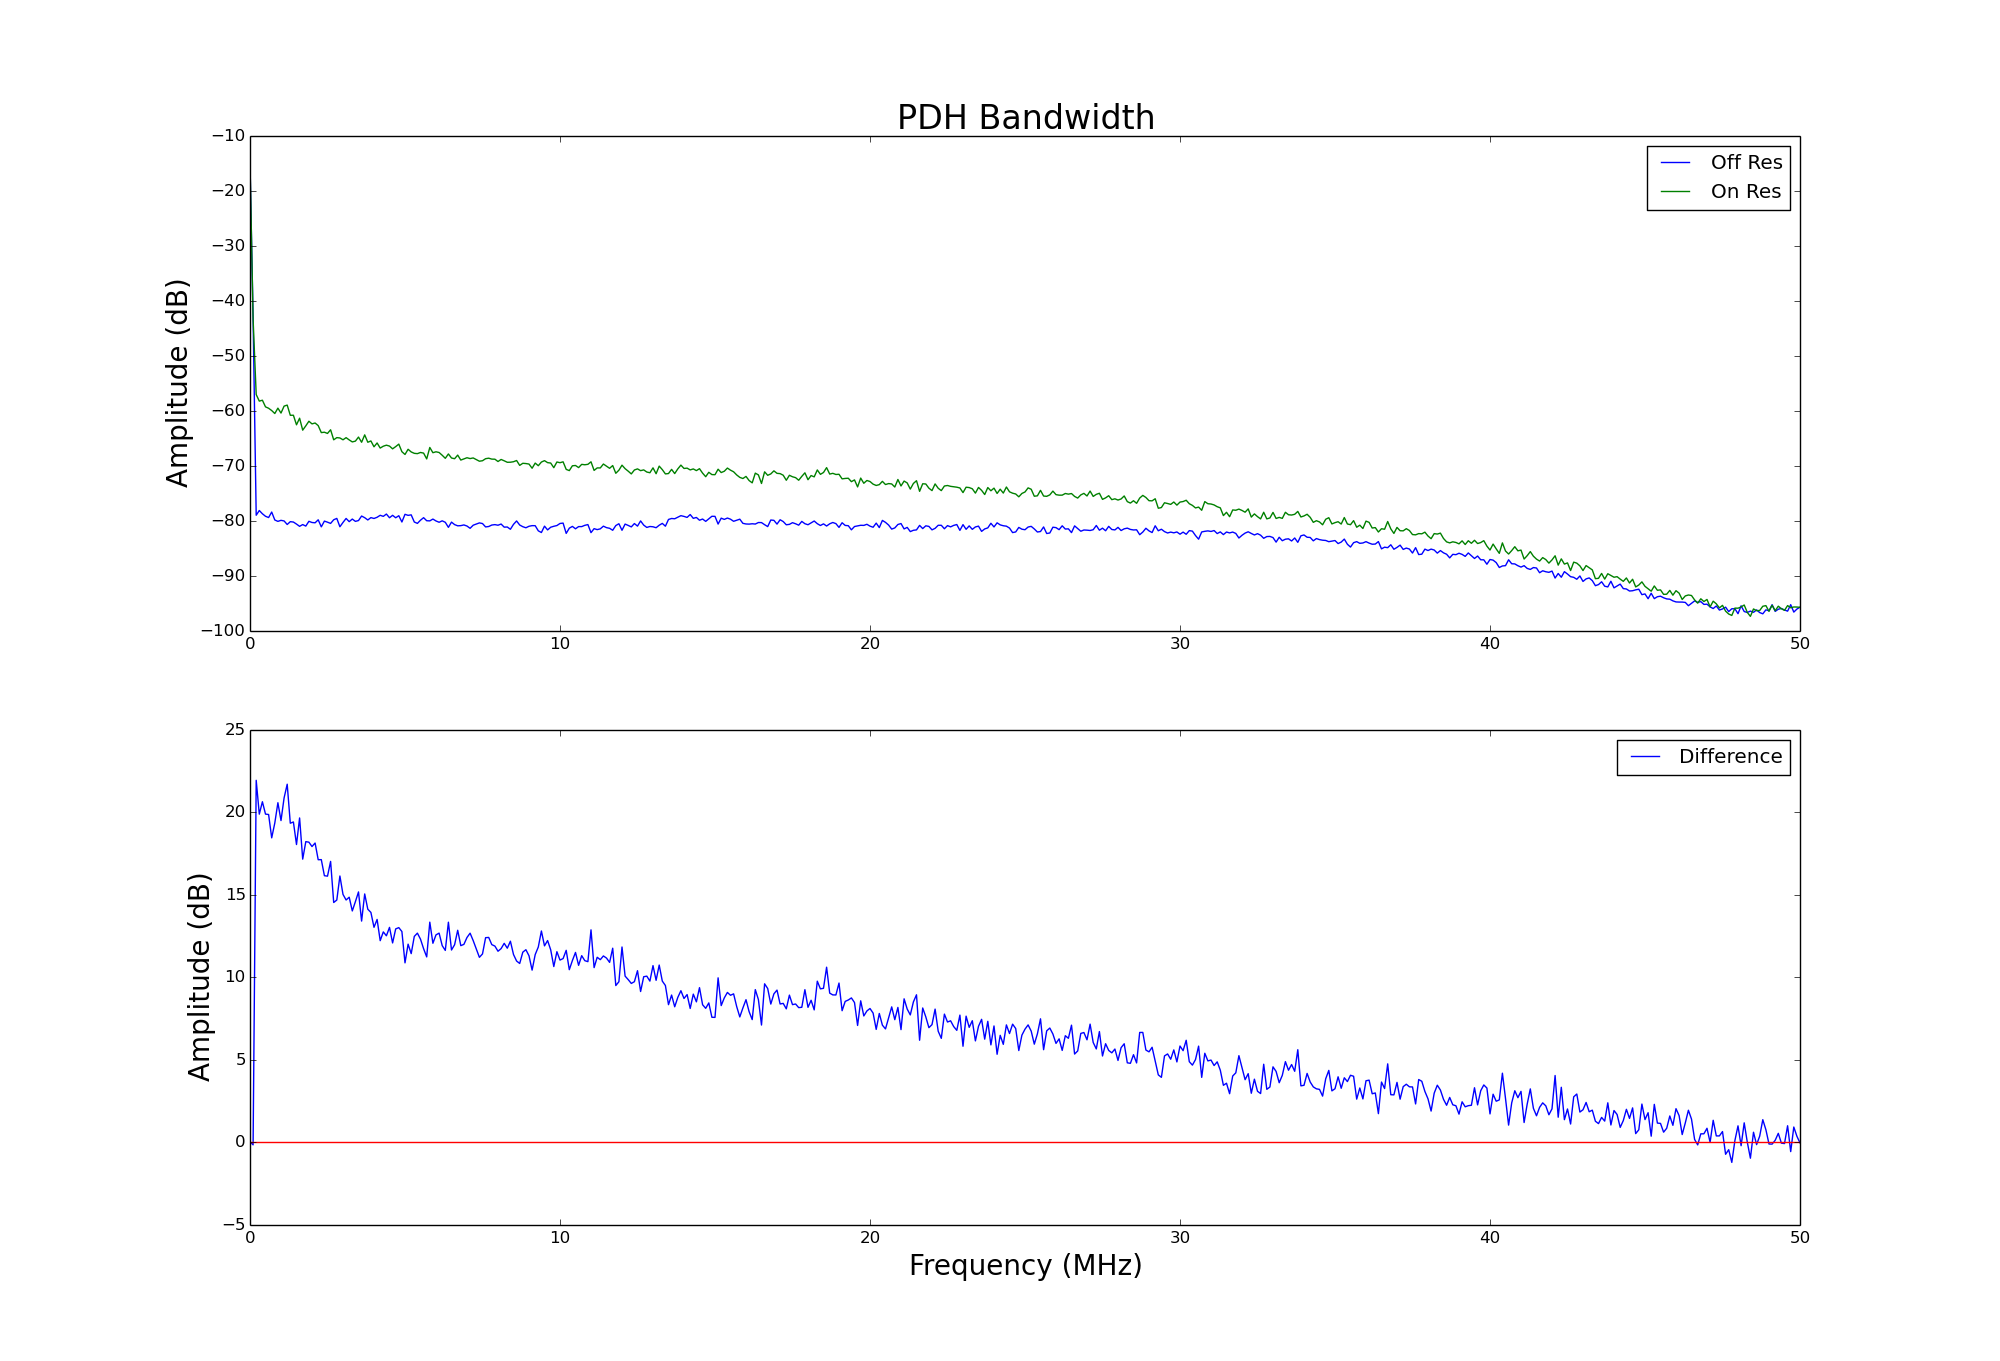
\includegraphics[width=\linewidth]{Figs/bandwidth_measurement.png}
    \captionof{figure}{Something something bandwidth.}
    \label{bandwidth_measurement}
\end{Figure}


\subsection{Linewidth Measurements}

{\color{red}Words are hard. The next explanation feels clumsy to me.}

By directing a locked laser's light through a high finesse cavity and either scanning the laser's frequency with an \gls{aom} or scanning the cavity's length with a piezo attached to one of the mirrors it is possible to get a trace of the convolution of the cavity's Airy transmission function T and the laser's lineshape L.

\begin{equation}
T(\delta) = \frac{1}{1+F sin^2(\delta)}
\end{equation}

\begin{equation}
L(\delta) = \frac{\sigma^2}{\delta^2 + \sigma^2}
\end{equation}

Where F is the coefficient of finesse for the cavitiy, $\delta$ is the frequency detuning of the laser from the cavity's resonance and $2\sigma$ is the \gls{fwhm} of the Lorentzian.

Convolving a cavity with a finesse of 20942 (which has a transmision function with a \gls{fwhm} of 71.6kHz) with a Lorentzian with a \gls{fwhm} of 10kHz produces an approximately Lorentzian line with a \gls{fwhm} of 81.6KHz as shown in figure \ref{convolution}.

\begin{Figure}
    \centering
    \captionsetup{type=figure}
    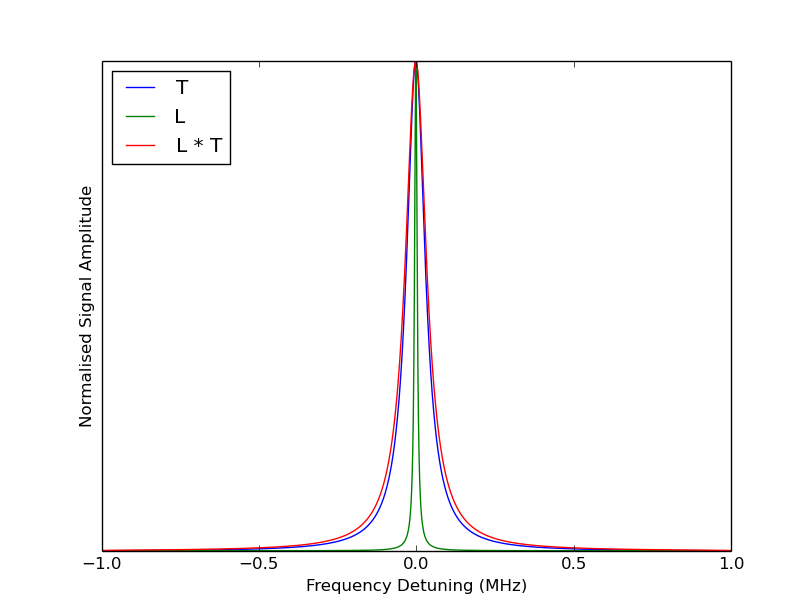
\includegraphics[width=\linewidth]{Figs/convolution.png}
    \captionof{figure}{The blue line shows the transmision function for a acvity with a finesse of 20942. The green line shows a Lorentzian with a \gls{fwhm} of 10kHz. The red line shows the convolution of the blue and green lines and represents the signal that would be measured as transmitting through a cavity illuminated by a laser with a lineshape given by the green line.}
    \label{convolution}
\end{Figure}

If, instead of scanning the laser the frequency is set so that the frequency is at a point where the the transmission through the cavity is partway up the side of the peak then the subsequent fluctuations in amplitude can be mapped to a Lorentzian fitted to the peak and thus transformed to a frequency. The distribution of frequencies in turn provide can be used to calculate the linewidth of the laser.

Using this technique linewidths of 11.72 kHz have been measured {\color{red}using the experimental setup described somewhere else in this document}.


\begin{Figure}
    \centering
    \captionsetup{type=figure}
    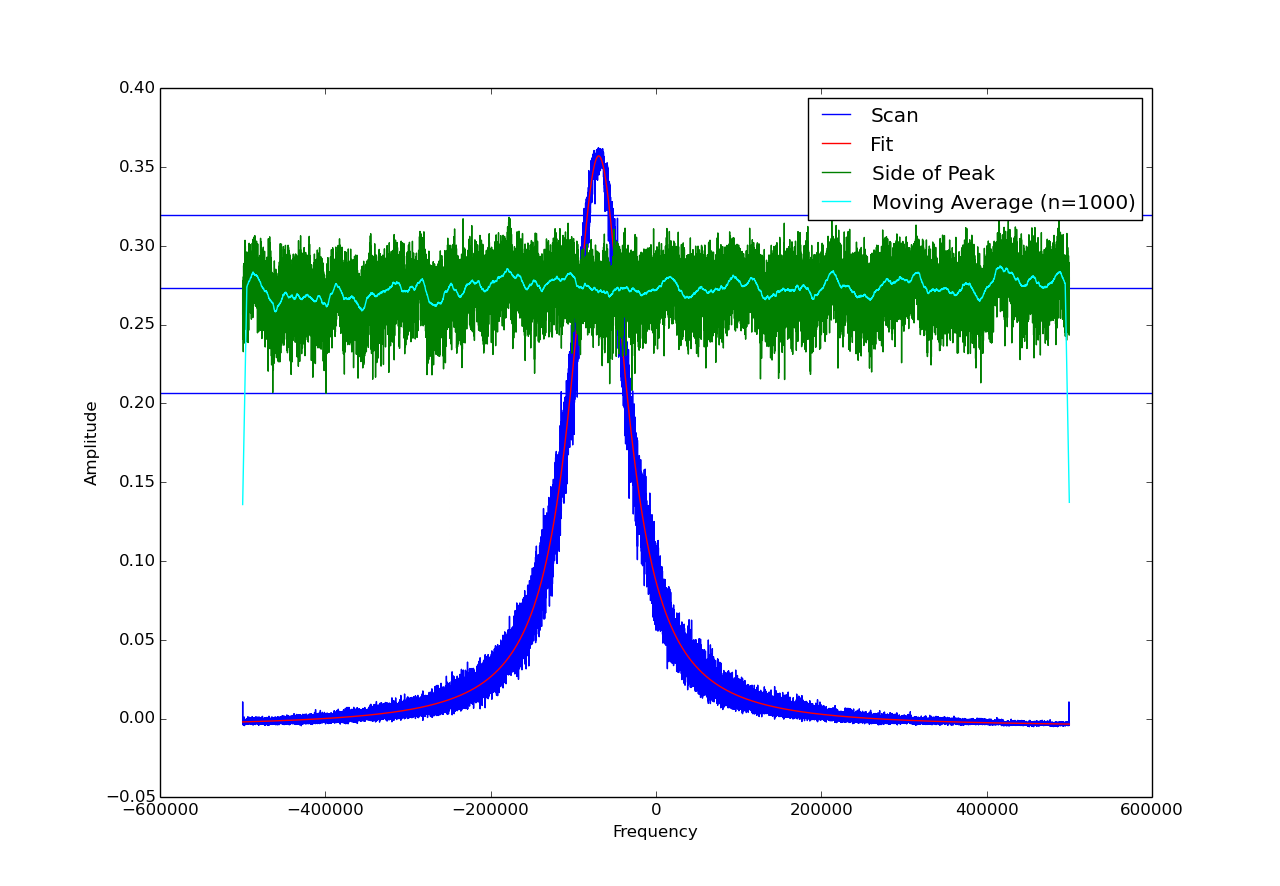
\includegraphics[width=\linewidth]{Figs/linewidth_measurement.png}
    \captionof{figure}{A polarisation spectroscopy locked laser scanned through a high finesse cavity (blue line). The green line is the same laser, no longer scanning, with it's frequency adjusted such that it is on the side of the transmission peak.}
    \label{linewidth_measurement}
\end{Figure}

\begin{Figure}
    \centering
    \captionsetup{type=figure}
    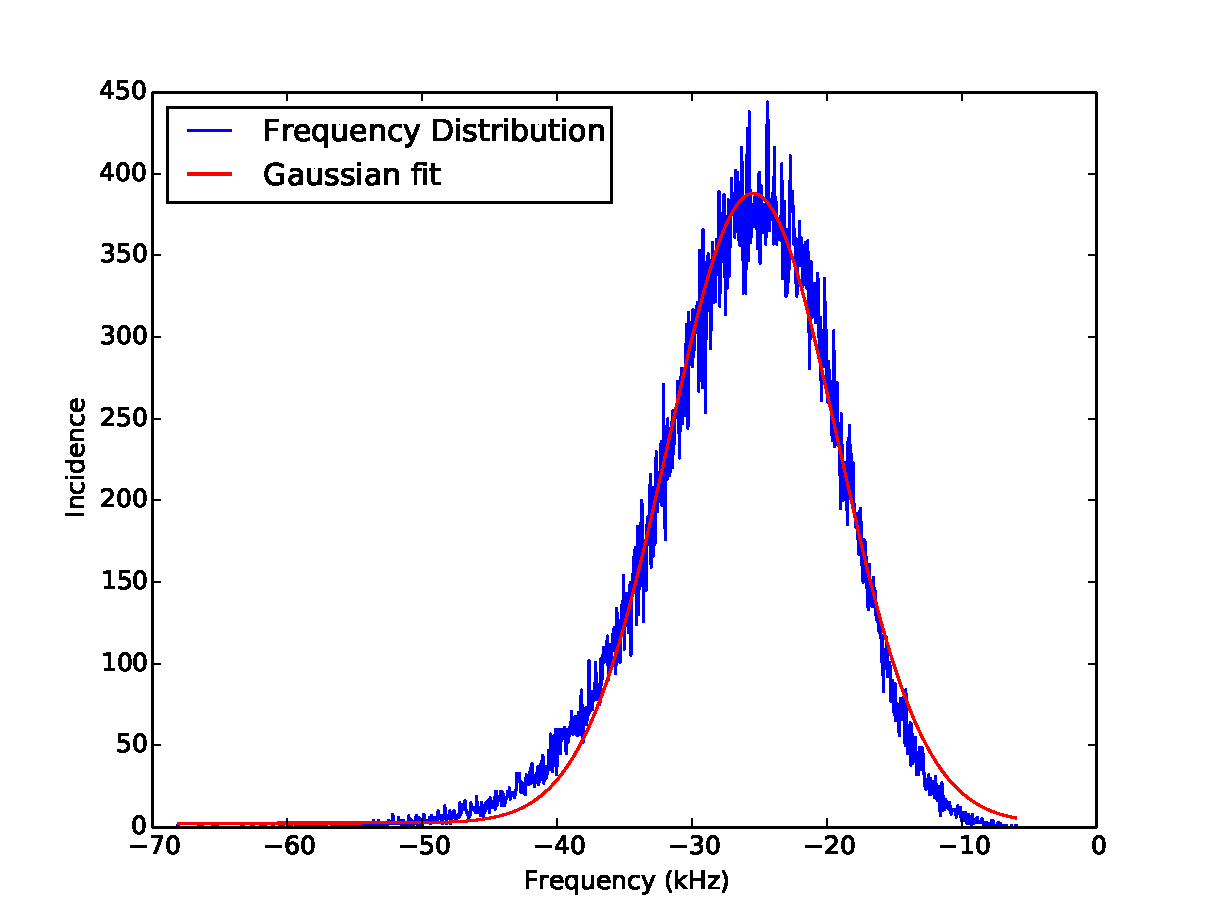
\includegraphics[width=\linewidth]{Figs/freq_distribution.pdf}
    \captionof{figure}{The blue line shows the frequency distribution of the feen line in figure \ref{linewidth_measurement}. The red line is a Gaussian fit which has a \gls{fwhm} of 11.72 kHz.}
\end{Figure}

\bibliographystyle{plain}
\bibliography{Library}

\end{multicols}
\end{document}
